Para o desenvolvimento deste trabalho foram dadas prioridade e
preferência para a utilização de um sistema embarcado de núcleo ARM,
com o intúito de desenvolver as capacidades de operar tal tecnologia
de processamento, trabalhando com sistema um eletrônico simples de fácil acesso mas que atenda as necessidades do projeto, bem como a utilização de ferramentas de uso livre.

Como metodologia foi adotado o procedimento de comparação de
resultados gerados entre uma técnica de controle bem estabalecida,
com uma lógica clássica utilizando um controlador
Proporcional+Integral (PI), e um controlador proposto
utilizando a LPA$E\tau$. 







\section{Materiais}

O protótipo físico foi constuído baseado em um microcontrolador da
família Texas Instruments, modelo $Tiva^{TM}$ TM4C123GH6PM, drive para
acionamento do tipo \emph{Pulse Width Modulation}(PWM) do motor com
circuito integrado de tecnologia CMOS (IRF540), motor de corrente
contínua acoplado a um disco compacto(CD), com uma etiqueta,
Figura \ref{fig:discoSensor}, para acionar o sensor óptico e servir de
indicador para contagem de giros do motor.
Fonte de alimentação chaveada de 12V 10W.
A maior parte do sistema pode ser visto na Figura \ref{fig:discoSensorGeral} .


\begin{figure}[!htb]
\center
\caption{Visão geral do sistema }
\subfloat[]{
	\label{fig:discoSensor}
	\includegraphics[scale=0.07, angle=0, clip=true, trim=300 200 1200 200]{./imagens/discoSensor.jpg}
	}
\subfloat[]{ 
	\label{fig:discoSensorGeral} 
	\includegraphics[scale=0.07, angle=0, clip=true, trim=300 200 400 200]{./imagens/discoSensorGeral.jpg} 
	}

{\small Figure: Próprio autor}
\end{figure}

As ferramentas de software utilizadas foram em sua totalidade de uso
livre ou de código aberto, sendo eles:

\begin{itemize}
\item Sistema Operacional GNU/Linux Debian 8(Jessie);
\item GNOME Shell;
\item Editores de texto e códigos fonte VIM e Emacs;
\item Compilador GCC para ARM (arm-none-eabi-gcc);
\item GNU Make;
\item Processador de texto \LaTeX - pdfTEX; 
\item Pacotes geradores de figuras TikZ, PGF e GNU pic(Groff);
\item Gerador de gráficos GNUPlot;
\item Teminal de comunicação Minicom;
\item Gravador para microcontrolador ARM LM4Flash.
\end{itemize}










\section{ Métodos }

Os métodos utilizados buscam mostrar como implementar e testar o
sistema de controle proposto, possibilitando uma posterior replicação
dos ensaios utilizados e análise da forma como o sistema foi
construído e testado.

%!@# rever frase completa
%Os métodos utilizados para a verificação do objetivo do projeto devem verificar quão próximo o resultado obtido empiricamente foi do objetivo esperado, de modo que as expectativas referentes aos objetivos propostos sejam atendidos ou sua 'negação' seja devidamente esclarecidas. 

Basicamente, são realizadas as seguintes etapas:

\begin{itemize}
\item Levantamento de um modelo matemático do sistema protótipo utilizado;
\item Verificação da qualidade desse modelo, com erro percentual médio
  menor do que 5\%, considerando um sistema não crítico. Se o erro
  percentual médio for maior do que os 5\%, retornar ao passo anterior e
  melhorar o modelo;
\item Definição dos requisitos de desempenho do sistema;
\item Realizar o controle utilizando um controlador PI;
\item Realizar o controle utilizando um controlador LPA$E\tau$;
\end{itemize}

\nomenclature{$PI$}{Proporcional-Integral}



\subsection{ Obtenção de um modelo matemático do processo }

A obtenção do modelo matemático do processo,
apresentada no anexo B, consiste em equacionar
regras matemáticas a partir da física básica do sistema,
de modo a obter uma função,
contemplando as as principais variáveis do sistema,
e que ajustadas adequadamente,
possam produzir um resultado semelhante ao comportamento do sistema
original, resultado empírico de funcionamento.



\subsection{ Qualidade do modelo }

Garantir uma boa qualidade ao modelo é importante para que se possa
utilizá-lo para calcular os parametros dos controladores.

A qualidade do modelo é relativa ao erro aceitável para o sistema estudado. Para o modelo obtido neste estudo foi aplicada o cálculo de Erro Relativo Percentual, e foram feitas análises em trechos diferentes em função da não linearidade inicial apresentada pelo comportamento do motor da planta em estudo.


A equação para o cálculo de Erro Relativo Percentual é:

\begin{equation}
 \% erro = \frac{| \text{\emph{valor real}} -\text{\emph{valor calculado}} |}{\text{\emph{valor real}}} x 100
\end{equation}

Realizando a somatória para o cálculo de erro médio com todas as
amostras a serem aquisitadas: 

\begin{equation}
 \% erro = \frac{100}{N} . \sum_{n = inicial}^{n = final} {\frac{| \text{\emph{r[n]}} -\text{\emph{c[n]}} |}{\text{\emph{r[n]}}} } 
\end{equation}


Onde:

\setlength{\parindent}{2cm}
r : valor real, empírico; 

c : valor calculado;

n : número da amostra aquisitada;

N : número total de amostras.




\subsection{ Requisitos de desempenho do sistema }

Os principais e mais comuns requisitos de desempenho dos sistemas são:

\begin{itemize}

\item Velocidade de resposta: A constante de tempo $\tau$ é a medida
  de tempo em que um sistema de primeira ordem alcança os $63\%$ do
  sinal máximo desejado, assumindo que para a estabilidade o sistema
  precisa de um tempo de cinco vezes o tempo do $\tau$. Assim, é
  definida como velocidade de resposta desejada uma estabilidade
  equivalente a duas vezes o  $\tau$, reduzindo a $\frac{2}{5}$ do valor
  inicial. 
%\item Velocidade de resposta: A Figura \ref{fig:acaoMalhaAberTau} mostra que para a constante de tempo $\tau$, foi registrado um intevalo de 2,5 segundos, assim, a estabilidade é alcançada em torno de 12,5 segundos, assumindo a partir daí o regime de estabilidade.
%Como requisito de desempenho é estipulada uma redução do tempo de resposta para $\frac{1}{2}$ do valor inicial, com o novo $\tau$ assimindo o valor máximo de 1,25 segundos.

\item Sobressinal: Para muitos sistemas ter um sobressinal elevado é algo completamente indesejado, outros permitem alguma oscilação, no caso aqui estudado é definido que o sobressinal aceitável é de no máximo $10\%$ do valor desejado.
  
\item Erro de regime estacionário: é a exatidão da resposta do sistema em relação ao valor desejado, assume-se um valor aceitável para o sistema, nesse caso não crítico, de $5\%$.
\end{itemize}



\subsection{ Ensaio com o controlador Liga/Desliga }

O controlador Liga/Desliga é o de mais fácil implementação, porém não
apresenta um controle muito eficiente. Consiste em acionar a carga
com 100$\%$ da alimentação até que a saída alcance o valor desejado,
desligando-a e retornando a ligá-la quando estiver abaixo do valor
desejado, ficando num ciclo de liga-desliga. 



\subsection{ Ensaio com o controlador PI }

A ação de controle Proporcional+Integral (PI) é adequada ao sistema
proposto utilizado neste estudo.

A Equação \ref{eq:metodoPI} descreve o controlador PI a ser implementado.

\begin{equation}
  u(t) = kp.e(t) + ki \int_{0}^{\infty} e(t) dt
\label{eq:metodoPI}  
\end{equation}


\subsection{ Ensaio com o controlador LPA$E\tau$ }

O controlador LPA$E\tau$ a ser implementado é mostrado na Figura 
\ref{fig:metodoControleLPAEt}, de modo que o $\mu_0 + \delta$ sejam
ajustados de acordo com a Tabela \ref{tab:correcaoDelta}, conforme
exposto no respectivo capítulo.

%%%%%%%%%%%%%%%%%%%%%%%%%%%%%%%%%%%%%%%%%%%%%% Fig
\begin{figure}[!h]%%%%%%%%%%%%%%%%%%%%%%%%%%%%%%%%
\centering
\caption{Representação do reticulado da LPA$E\tau$ para o controlador}
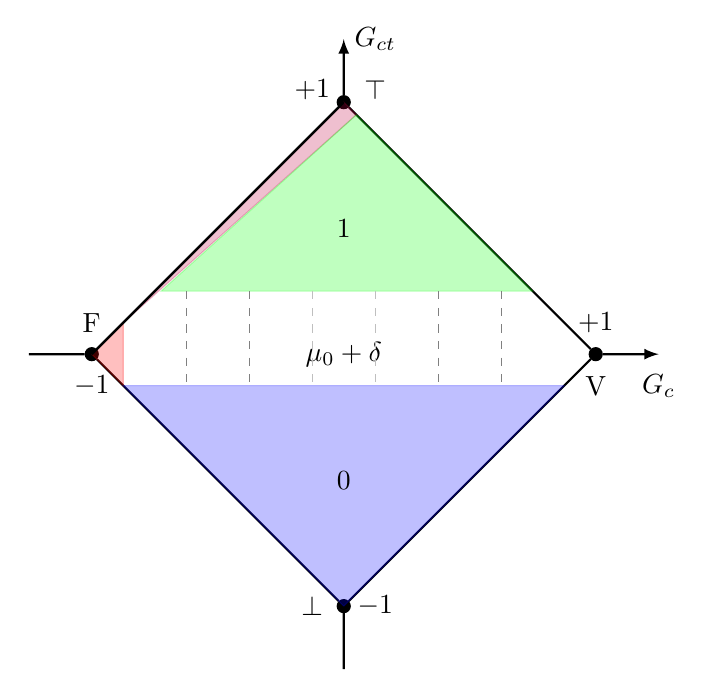
\begin{tikzpicture}[scale=0.80]
\tikzset{ >=latex, inner sep=0pt, outer sep=0pt,  }

%\draw [lightgray, dashed](0,0) grid (10,10);

\node [fill=black, circle] (V) at (9,5) {:};
\node [fill=black, circle] (F) at (1,5) {:};
\node [fill=black, circle] (T) at (5,9) {:};
\node [fill=black, circle] (L) at (5,1) {:};

\draw [->, thick] (V)   -- (10,5);
\draw [    thick] (0,5) -- (F);
\draw [->, thick] (T)   -- (5,10);
\draw [    thick] (5,0) -- (L);

\draw [thick] (V) -- (T);
\draw [thick] (T) -- (F);
\draw [thick] (F) -- (L);
\draw [thick] (L) -- (V);

\node at (10,4.5) {$G_{c}$};
\node at (5.5,10) {$G_{ct}$};

\node at (4.5,9.2) {$+1$};
\node at (9.0,5.5) {$+1$};
\node at (5.5,1.0) {$-1$};
\node at (1.0,4.5) {$-1$};

\node at (9.0,4.5) {V};
\node at (1.0,5.5) {F};
\node at (5.5,9.2) {$\top$};
\node at (4.5,1.0) {$\bot$};

\draw [fill, red,nearly transparent] (1.0,5.0) -- (1.5,5.5) -- (1.5,4.5) -- (1.0,5.0);
\draw [fill, purple, nearly transparent] (1.5,5.5) -- (5.0,9.0) -- (5.2,8.8) -- (1.5,5.5);
\draw [fill, blue, nearly transparent] (5.0,1.0) -- (8.5,4.5) -- (1.5,4.5) -- (5.0,1.0);
\draw [fill, green, nearly transparent] (5.2,8.8) -- (2.1,6.0) -- (8.0,6.0) -- (5.2,8.8);

\draw [thick] (5.0,9.0) -- (1.0,5.0);

\node at (5.0,7.0) {1};
\node at (5.0,5.0) {$\mu_0 + \delta$};
\node at (5.0,3.0) {0};

\draw [dashed, gray] (2.5,6.0) -- (2.5,4.5);
\draw [dashed, gray] (3.5,6.0) -- (3.5,4.5);
\draw [dashed, gray] (6.5,6.0) -- (6.5,4.5);
\draw [dashed, gray] (7.5,6.0) -- (7.5,4.5);
\draw [dashed, lightgray] (4.5,6.0) -- (4.5,4.5);
\draw [dashed, lightgray] (5.5,6.0) -- (5.5,4.5);

\end{tikzpicture}
\label{fig:metodoControleLPAEt}

{\small Fonte: Próprio autor }
\end{figure}
%%%%%%%%%%%%%%%%%%%%%%%%%%%%%%%%%%%%%%%%%%%%%%%%%%






